%!TEX program = lualatex
\documentclass[border=0mm,11pt]{standalone}
%\usepackage{color}
%\usepackage{tikz}
\usepackage[T1]{fontenc}
\usepackage[sc]{mathpazo}
\usepackage{tikz-feynman}
\tikzfeynmanset{compat=1.1.0}


\begin{document}

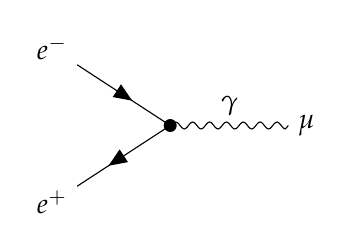
\begin{tikzpicture}[]
    \begin{feynman}
    \vertex (fant);
    \vertex [above =of fant, xshift=0.0cm, yshift=-0.792cm] (f1) {$e^{-}$};%-1.792
    \vertex [below =of fant, xshift=0.0cm, yshift=0.792cm] (f2) {$e^{+}$};
    \vertex [right=of fant, xshift=0.0cm, yshift=0.0cm] (a);
    \vertex [right=of a, xshift=0.0cm, yshift=0.0cm] (b) {$\mu$};
    \node [dot] at (a) {};
    \diagram* {
    (f1) -- [fermion] (a) -- [photon, edge label=\($\gamma$\)] (b),
    (f2) -- [anti fermion] (a),
    };
    \end{feynman}
\end{tikzpicture}

\end{document}